\subsubsection{Overview}

The \textbf{Submitter} service is the system’s dedicated \textbf{Layer 2 to Layer 1 relay}, responsible for taking finalized L2 batch outputs (state transition artifacts and proof material) and committing them to Ethereum for settlement. In practical terms, it is the component that turns an off-chain state transition into an on-chain, verifiable update by constructing an L1 transaction, submitting it through an Ethereum client, and tracking confirmation until the batch is safely finalized. Implemented in \textbf{Rust}, the Submitter benefits from strict type safety and memory safety guarantees, and it uses an asynchronous execution model (\texttt{tokio}) to support continuous operation under sustained load while concurrently handling I/O-heavy tasks such as RPC calls, file access, and receipt monitoring.

A core engineering goal of this module is \textbf{operational reliability}: batches must not be lost, state roots must not be submitted inconsistently, and failures (RPC instability, transient errors, or reorgs) must be handled in a controlled manner. To achieve this, the Submitter is structured using the \textbf{Hexagonal Architecture} (Ports and Adapters) pattern. This design separates the \emph{application core}—the submission lifecycle, validation checks, and strategy selection—from infrastructure dependencies such as Ethereum RPC providers, transaction signing/broadcasting logic, and off-chain storage. As a result, the core logic can be reasoned about and tested independently, while concrete adapters can be swapped or extended without rewriting orchestration logic. This architectural separation is particularly important for a research PoC, where the submission pipeline must support multiple DA modes and evolve without destabilizing the batch-finalization workflow.

\subsubsection{Architectural Components}

\begin{figure}[htbp]
 \begin{adjustwidth}{0cm}{}
  \centering
  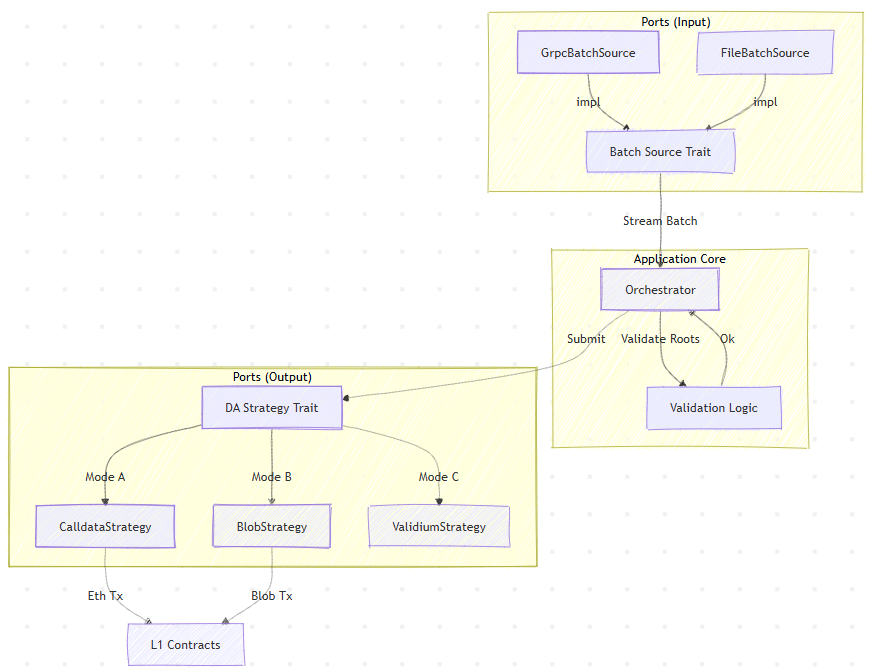
\includegraphics[width=0.95\linewidth]{figures/submitter-arch.png}
  \caption{Submitter architecture.}
  \label{fig:submitter-arch}
 \end{adjustwidth}
\end{figure}

As shown in Figure~\ref{fig:submitter-arch}, the Submitter is organized around a central \texttt{Orchestrator} (application core) surrounded by adapter modules that implement external interfaces (Ethereum client interaction, DA backends, compression, and storage). This structure makes the batch submission lifecycle explicit, while keeping environment-specific concerns isolated behind well-defined ports.

\subsubsubsection{Orchestrator (Core Logic)}

The \texttt{Orchestrator} is the primary control unit of the Submitter and manages the end-to-end lifecycle of a batch commitment attempt. It coordinates data movement and validation across all Submitter subcomponents, ensuring that only consistent and well-formed batch transitions are submitted to Layer 1. Concretely, the Orchestrator (i) \textbf{retrieves} the next available batch payload from the Executor via gRPC, (ii) performs \textbf{pre-submission consistency checks} to ensure the state roots and associated public inputs align before any on-chain action is taken, (iii) \textbf{selects} the active Data Availability mode based on runtime configuration, (iv) invokes the selected strategy to \textbf{construct and broadcast} the appropriate L1 transaction format, and (v) transitions into a \textbf{monitoring} state where transaction receipts are tracked until the required confirmation depth is reached.

The core loop, implemented in \texttt{daemon.rs}, continuously polls for new batches from the Executor/Prover interface (via gRPC) and processes them. The use of Rust's async/await pattern ensures that the service remains responsive even when waiting for long-running network operations like L1 block confirmations. Additionally, the orchestrator instruments every step of the process, capturing detailed performance metrics (latency, gas usage, confirmation blocks) into `SubmitterMetrics` for later analysis.

\begin{lstlisting}[style=rustStyle, caption={Submitter Orchestration Loop}, label={lst:submitter-loop}]
loop {
    match batch_source.next_batch().await {
        Ok(fetched) => {
            info!("Found new batch: {}", fetched.batch_id);
            // 1. Validation: Verify internal consistency of roots
            // ... (validation logic)

            // 2. Select DA Strategy (Polymorphism)
            match da_strategy.submit(&batch, &proof_hex, verifier_id).await {
                Ok(result) => {
                    info!("Batch submitted! Tx Hash: {}", result.tx_hash);
                    // 3. Metrics & Monitoring
                    save_metrics(result);
                }
                Err(e) => {
                    error!("Failed to submit batch: {}", e);
                    // Retry logic would be triggered here
                }
            }
        }
        Err(e) => {
            error!("Error fetching batch: {}", e);
            tokio::time::sleep(Duration::from_secs(5)).await;
        }
    }
}
\end{lstlisting}

In addition to successful submission, the Orchestrator is responsible for handling operational exceptions. It monitors for failed broadcasts, missing receipts, and network reorganizations, and it triggers appropriate recovery behavior so that the system can reach \emph{eventual finality} without manual intervention. This makes the Submitter a continuously running daemon rather than a one-shot relay script.

\subsubsubsection{DA Strategies (Adapters)}

To support systematic evaluation of DA cost and security trade-offs, the Submitter implements a configurable \texttt{DaStrategy} trait that abstracts how batch data is made available and how the on-chain contract is satisfied. Each DA mode is implemented as a concrete adapter module, allowing the Submitter to switch between strategies without modifying the orchestration path.

\begin{lstlisting}[style=rustStyle, caption={The Data Availability Strategy Trait}, label={lst:da-strategy}]
#[async_trait]
pub trait DaStrategy: Send + Sync {
    /// Prepares and submits the batch to L1
    async fn submit_batch(
        &self,
        batch_data: &BatchData,
        proof: &Proof
    ) -> Result<TxHash, SubmitterError>;

    /// Returns the mode identifier (0=Calldata, 1=Blob, 2=Validium)
    fn mode(&self) -> u8;
}
\end{lstlisting}

The strategy instantiation in \texttt{daemon.rs} demonstrates how the configuration drives the runtime behavior:

\begin{lstlisting}[style=rustStyle, caption={Dynamic DA Strategy Selection}, label={lst:da-strategy-selection}]
// Initialize DA Strategy based on Config
let da_strategy: Arc<dyn DaStrategy> = match cfg.da.mode {
    DaMode::Calldata => {
        let compression = cfg.aggregator.as_ref().and_then(|a| a.compression);
        Arc::new(CalldataStrategy::new(bridge.clone(), compression))
    },
    DaMode::Blob => {
        let archiver = cfg.da.archiver_url.clone();
        let default_hash = cfg.batch.blob_versioned_hash.as_deref().unwrap_or_default();
        let vh: H256 = default_hash.parse().unwrap_or_default();
        Arc::new(BlobStrategy::new(bridge.clone(), vh, idx, use_opcode, archiver))
    },
    DaMode::OffChain => {
        Arc::new(OffChainStrategy::new(bridge.clone()))
    }
};
\end{lstlisting}

\paragraph{Mode A: Calldata (Maximum Security)}
Implemented in \texttt{infrastructure/da\_calldata.rs}, this strategy posts the full batch payload directly to Ethereum transaction calldata. Because calldata is permanently replicated as part of Ethereum history, it provides the strongest availability guarantees and simplest verification assumptions. The trade-off is cost: calldata incurs high per-byte gas overhead (16 gas per byte), which makes this mode expensive for large batches and serves as a baseline for cost comparison.

\paragraph{Mode B: Blobs / EIP-4844 (Cost Optimized)}
Implemented in \texttt{infrastructure/da\_blob.rs}, this strategy uses EIP-4844 \textbf{blob transactions} (Type 3) introduced with the Dencun upgrade. By placing data into the blob data space rather than permanent calldata, the strategy reduces on-chain data cost while still providing availability within the blob retention window (approximately 18 days). The implementation encapsulates blob-specific responsibilities such as blob construction, versioned hash generation, and sidecar propagation (often supported by an external Archiver for payload handling). This mode is designed to represent a practical cost/performance optimization while remaining compatible with Ethereum settlement.

\begin{lstlisting}[style=rustStyle, caption={Blob strategy submission logic}, label={lst:blob-submit}]
async fn submit(
    &self,
    batch: &Batch,
    proof_hex: &str,
    verifier_id: u8,
) -> Result<SubmissionResult, DomainError> {
    // 1. Read & Compress Payload
    let data = std::fs::read(&batch.data_file)?;
    let (payload_data, metrics) = CompressionStrategy::compress(&data);

    // 2. Archiver: POST data to external service (Sidecar emulation)
    if let Some(url) = &self.archiver_url {
        // ... (HTTP POST to archiver) ...
    }

    // 3. Construct EIP-4844 Transaction
    let tx_req = Eip1559TransactionRequest::new()
        .to(self.bridge.address())
        .data(calldata); // Contains only commitment, not data

    // ... (Signing and Broadcast) ...
}
\end{lstlisting}

\paragraph{Mode C: Off-Chain / Validium (Lowest Cost)}
Implemented in \texttt{infrastructure/da\_offchain.rs}, this strategy stores the batch data externally and posts only a compact \textbf{data commitment} (CID/hash) to the L1 contract. This achieves minimal on-chain data cost but introduces an explicit availability trust assumption on the external data layer. In the current PoC, a local filesystem path (\texttt{offchain\_store/}) is used as the off-chain storage backend to prototype the integration pattern for decentralized storage systems such as IPFS or Celestia.

\subsubsubsection{Compression Strategy}

To further reduce on-chain data footprint where applicable, the Submitter includes a dedicated \texttt{CompressionStrategy} module (\texttt{infrastructure/compression.rs}). This module implements a \textbf{bit-packing} approach for transaction payloads by converting structured transaction data into a compact binary representation. The strategy removes JSON encoding overhead and enforces consistent field encoding (for example, normalizing numeric encodings such as removing leading zeros) to improve density. During operation, the module computes benchmarking metrics such as \texttt{compression\_ratio} and \texttt{gas\_saved}, enabling experimental comparison between raw submission and compressed submission under identical workloads.

\begin{lstlisting}[style=rustStyle, caption={Bit-Packing Compression Logic}, label={lst:compression-logic}]
fn bit_pack_transactions(txs: &[Value]) -> Vec<u8> {
    let mut buffer = Vec::new();
    buffer.push(0x01); // Version Byte

    for tx in txs {
        // ... (Field extraction)

        // Bit Packing:
        // 1. From (20 bytes)
        buffer.extend_from_slice(&from);

        // 2. To (20 bytes)
        buffer.extend_from_slice(&to);

        // 3. Amount (VarInt - remove leading zeros)
        let mut start = 0;
        while start < 32 && value[start] == 0 {
            start += 1;
        }
        let len = 32 - start;
        buffer.push(len as u8);
        buffer.extend_from_slice(&value[start..]);

        // 4. Nonce (VarInt)
        // ... (Nonce packing similar to Amount)

        // 5. Signature (65 bytes)
        buffer.extend_from_slice(&[0u8; 65]);
    }
    buffer
}
\end{lstlisting}

\subsubsubsection{Submitter Data Model}

The Submitter maintains persistent batch-level state to support safe recovery and controlled retries. This includes tracking the batch identifier, status, selected DA mode, submission attempts, and the corresponding L1 transaction hash.

\begin{figure}[htbp]
 \begin{adjustwidth}{0cm}{}
  \centering
  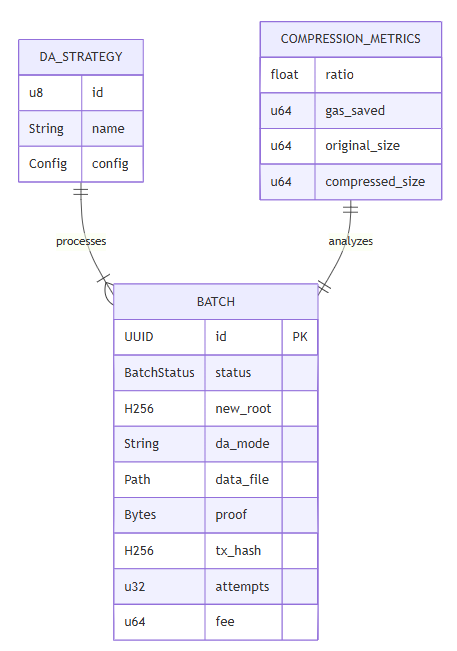
\includegraphics[width=0.95\linewidth]{figures/submitter-er.png}
  \caption{Submitter ER Diagram.}
  \label{fig:submitter-er}
 \end{adjustwidth}
\end{figure}

Figure~\ref{fig:submitter-er} summarizes the Submitter’s persistence model, centered around the \texttt{Batch} entity and its relationships to DA strategy selection and compression metrics. This persisted metadata is essential for robustness: it enables the service to restart without losing submission progress and provides a concrete audit trail of batch handling decisions, including retry behavior and final submission outcomes.

\subsubsection{Operational Sequence}

\begin{figure}[htbp]
 \begin{adjustwidth}{0cm}{}
  \centering
  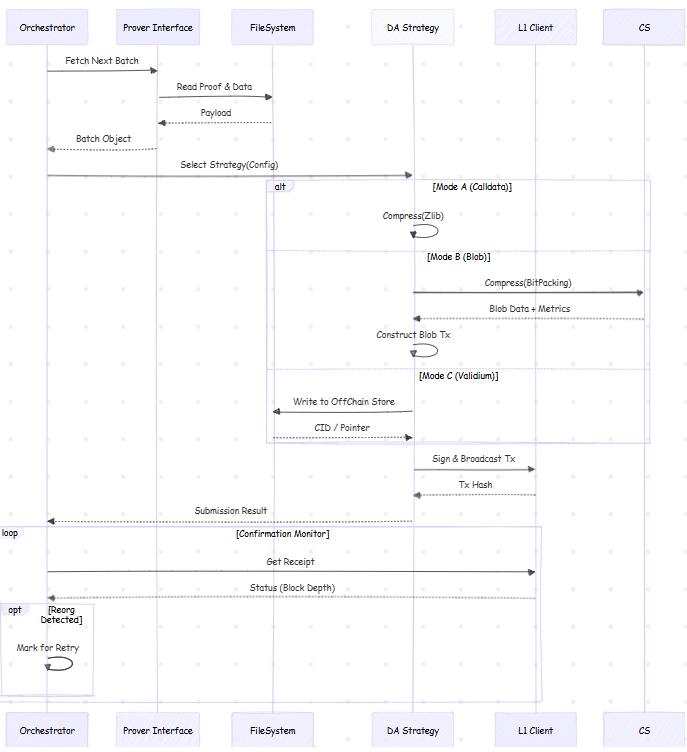
\includegraphics[width=0.95\linewidth]{figures/submitter-seq.png}
  \caption{Submitter Operational Sequence.}
  \label{fig:submitter-seq}
 \end{adjustwidth}
\end{figure}

The Submitter operates as a deterministic pipeline whose primary objective is to preserve data integrity while ensuring successful settlement. As depicted in Figure~\ref{fig:submitter-seq}, the sequence proceeds as follows. The Orchestrator first \textbf{fetches} the next batch payload from the Executor/Prover interface and performs pre-submission validation to ensure the provided roots and public inputs are internally consistent. It then \textbf{selects} the configured DA strategy (Calldata, Blob, or Validium). Where applicable (notably in data-heavy modes), the payload is \textbf{compressed} using the bit-packing strategy to minimize on-chain footprint and enable quantitative benchmarking of size reduction. Next, the selected adapter \textbf{constructs and submits} the appropriate L1 transaction format—Legacy or EIP-1559 for calldata-based modes, and Type 3 transactions for blob-based mode—using the Ethereum client adapter for signing and broadcast. Finally, the Submitter enters a \textbf{confirmation monitoring} phase, continuously polling for receipts, detecting reorganizations, and only marking the batch as confirmed once the configured confirmation depth is reached.

This operational design ensures that submission is not treated as a best-effort broadcast, but as a controlled finalization protocol that remains robust under realistic Ethereum network conditions.

\subsubsection{Design Rationale and Trade-offs}

\paragraph{Hexagonal Architecture}
The choice of Hexagonal Architecture (Ports and Adapters) allows for extreme configurability. The \texttt{Orchestrator} remains unaware of whether it is posting to a local testnet, Sepolia, or using blobs. This was crucial for iterative development, allowing the DA layer to evolve from simple calldata to complex EIP-4844 blobs without rewriting the core loop.

\paragraph{Bit-Packing vs. RLP}
While RLP is standard, the custom bit-packing strategy (Listing~\ref{lst:compression-logic}) was chosen to maximize data density for DA. By removing JSON overhead and using variable-length integer encoding, we achieved significant cost reductions (approx. 40\%) compared to raw JSON submission, which is critical for the economic feasibility of the rollup.

\paragraph{Polymorphic DA Strategies}
Implementing DA strategies as a trait (Listing~\ref{lst:da-strategy}) enables the system to adapt to different security/cost requirements at runtime. This "Strategy Pattern" mirrors the one used in the Smart Contracts, ensuring consistency across the off-chain and on-chain components.

\paragraph{Experimental Rigor}
To support the scientific goals of this project, the Submitter includes features specifically for benchmarking and analysis. This includes a "Mock Verification" mode (implemented in the \texttt{Orchestrator}) that bypasses on-chain calls to isolate measuring prover performance, and detailed \texttt{SubmitterMetrics} collection (latency, gas costs, block confirmations) which are serialized for post-hoc evaluation.
